\newpage
\section{Test results}\label{test_results}
This chapter presents the results of the test cases performed in Chapter 4. The test was conducted in an enterprise environment. All test participants use \ac{SaaS} products in their daily work. A total of 22 test runs were performed. These were divided equally between the two test systems. \\
Test candidates try to fill as many different positions as possible. This helps to give a more general meaning to the data obtained. Table \ref{tab:test_candidates} gives an overview of the selected test candidates. \\
\begin{table}[ht]
    \centering
    \begin{tabular}{|p{0.4\linewidth} | p{0.1\linewidth}|p{0.1\linewidth}|}
        \hline
        \textbf{Role} &\textbf{Normal}&\textbf{\ac{SDS}} \\ \hline
        Software Engineer & 7 & 4 \\ \hline
        Cusomer Success & 0 & 2 \\ \hline
        Intern & 1 & 0 \\ \hline
        Consultant & 0 & 1 \\ \hline
        Product Manager & 1 & 0 \\ \hline
        Customer Support & 1 & 0 \\ \hline
        Operation Manager & 0 & 1 \\ \hline
        Engineering Manager & 0 & 1 \\ \hline
        Director Engineering & 0 & 1 \\ \hline
        Customer Success Engineer & 1 & 0 \\ \hline
        IT Support Engineer & 0 & 1 \\ \hline \hline
        \textbf{Total} & 11 & 11 \\ \hline
    \end{tabular}
    \caption{\label{tab:test_candidates} Test candidates}
\end{table}

The list contains various positions from operational and lower management, but also some test candidates from higher management. Unfortunately, the majority of the test candidates are from the software development department, which could be related to the relationships of the author of this elaboration. \\

\subsection{Observation}
As a first step, this elaboration provides the test results of the observation of the test runs. These observations were carried out subjectively and provided information about the test candidates' reactions when dealing with the two systems.\\
Participants took a long time to reach the home page in every other test run. This user behavior shows that the distraction page works well. After the test run, participants indicated in the feedback session that they would move faster if they did not know this was a test. Overall, participants who took a long time on the home page stopped reading and immediately scrolled to the top of the page to get to the data table. There were no differences in interaction between the SDS testing system and the regular system. \\
As with the long distraction, participants show a pattern of quickly finding the "Add +" button to add a new entry in both applications. As with the long distraction, participants show the pattern of quickly finding the "Add" button in both applications to add a new entry. Then, participants continue adding data to the form without responding to the second view. Observation shows that there is one more entry in the normal application than in the \ac{SDS} application, which the test user cycled through the test application quickly. However, the notes show they were relatively even in their cycle time.  \\
Summarizing the observations when adding the data to the table, it seems that entering the data into the normal system was faster. Users quickly enter the data into the form and submit the form immediately. Furthermore, none of the participants ever asked for values for the status because the field was left open as a text box instead of offering a drop-down list. In comparison, two participants in the \ac{SDS} implementation application ask for preset values for status on the form. Of course, the selecting participants could also relate to this phenomenon.  \\
All in all, the observations of the test runs show no decisive differences between the two systems. However, one interaction that stood out in both applications was the tryout pattern instead of reading through the text or navigation bar elements. Instead, the user tried clicking on every element, resulting in a quick run through the test application but showing that \ac{SaaS} products should be intuitive. 

\subsection{Measurements}
This chapter presents the insights from the measurements taken during the test runs. These measurements can confirm the subjective observations made earlier. With the help of the measurement points presented in Chapter \ref{text_case}, it is possible to analyze the data collected. For example, if we take the duration between two measurement points, we obtain three timeslots. 
\begin{enumerate}
    \item \textbf{Find data table}: Starting the test - see the data table
    \item \textbf{Find add button}: See data table - see data add form
    \item \textbf{Add data to table}: See data add forme - submit data add form
\end{enumerate}
With the help of the measurements, it is possible to draw diagrams to understand the collected data better. One problem encountered when looking at the data is that the total duration of each run varies from run to run. A transformation with the collected data ensures that all results are comparable. In detail, the transformation calculates each duration slot relative to the total duration. All sections together result in a total percentage of 100\%. \\

With the prerequisites explained, it is time to look at the data. Starting with the measurements of the test runs on the application without \ac{SDS}.\\

\begin{figure}[htbp]
    \centerline{
    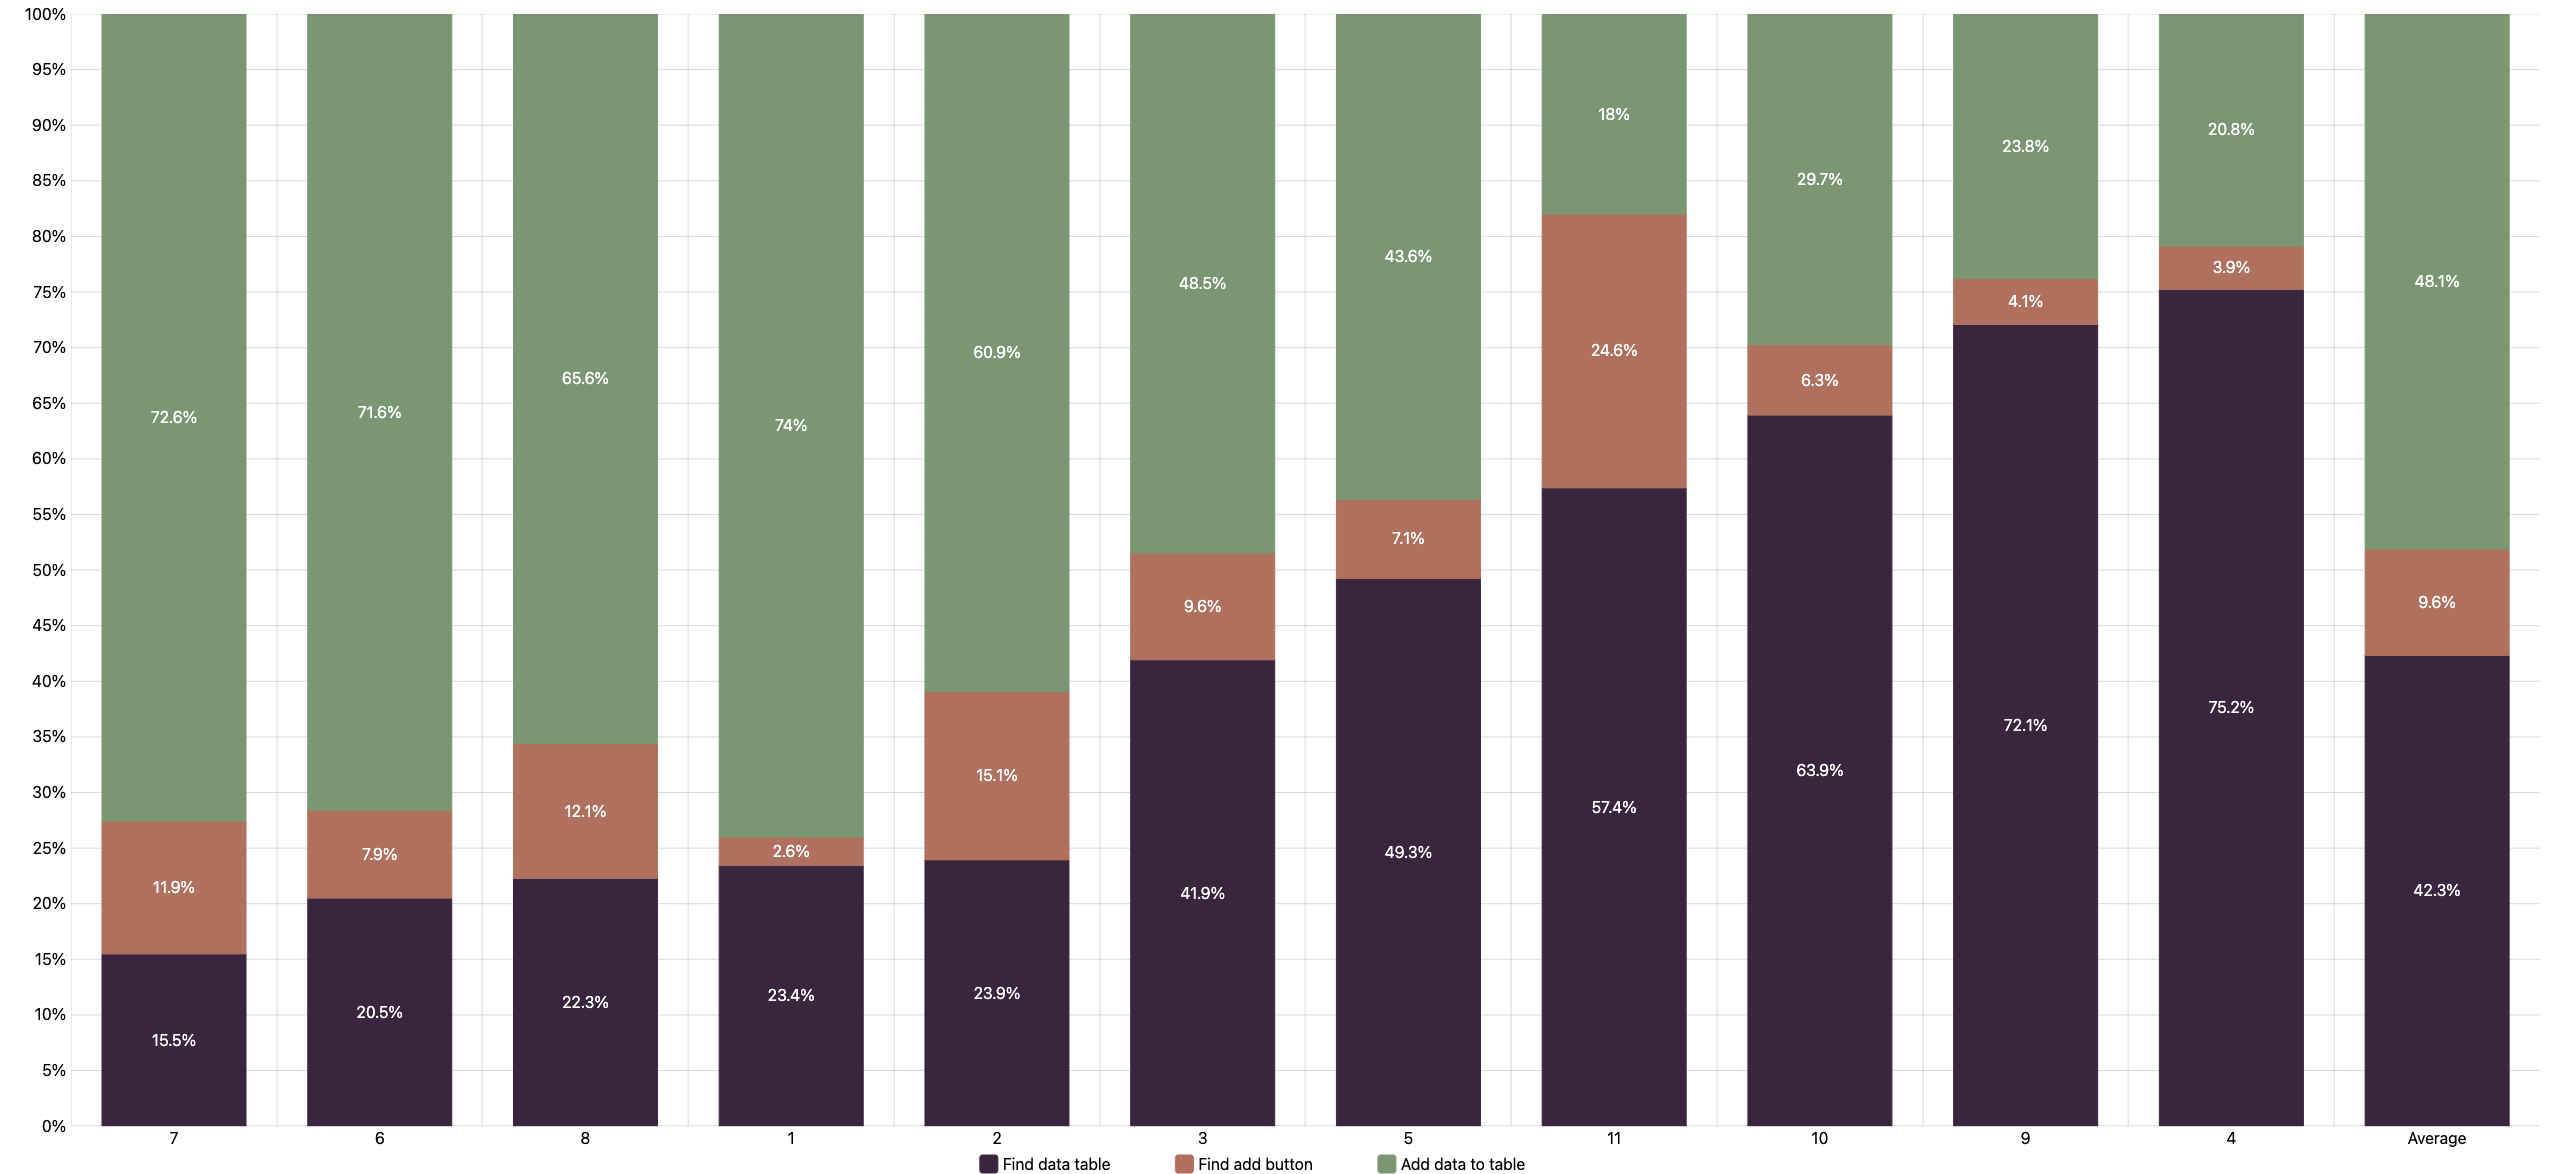
\includegraphics[width=\linewidth]{images/normal_test_data_chart.png}}
\caption{Chart of normal test data}
\label{test_data_normal}
\end{figure}
The chart in Figure \ref{test_data_normal} shows that the data confirms the point made in the observations. Sorted by time to find the data table, the chart shows the distribution of time needed. The first five columns show runs that the users completed test runs very quickly. As a result, data entry takes a relatively long time since typing slows down the user. A look at the end of the chart shows the long runs with a longer time on the home page. \\
The last column of the chart shows the average of all datasets combined. Once again, it is essantial to note that the average time spent on the distribution of finding the data table and adding data through the form is about the same. \\
The only breakout from the schema is the test run 11. In this run, the relative number shows that finding the "Add +" button, i.e., showing the data table, took longer than adding the data. A look at the data shows that this was one of the longer test runs of the data set, lasting almost two minutes. The long time taken indicates that the test user either interacted cautiously with the test application or had trouble navigating. \\
The data chart concludes that there are no surprises in the test runs for the application without SDS. It generally confirms the previously reported observation.\\

As a next step, the elaboration deals with the results of the test run of the application with implemented SDS. Expecting to see roughly the same distribution pattern of test data.  As in Figure \ref{test_data_normal}, this chart shows the relative time windows calculated using the total time required for each run. \\

\begin{figure}[htbp]
    \centerline{
    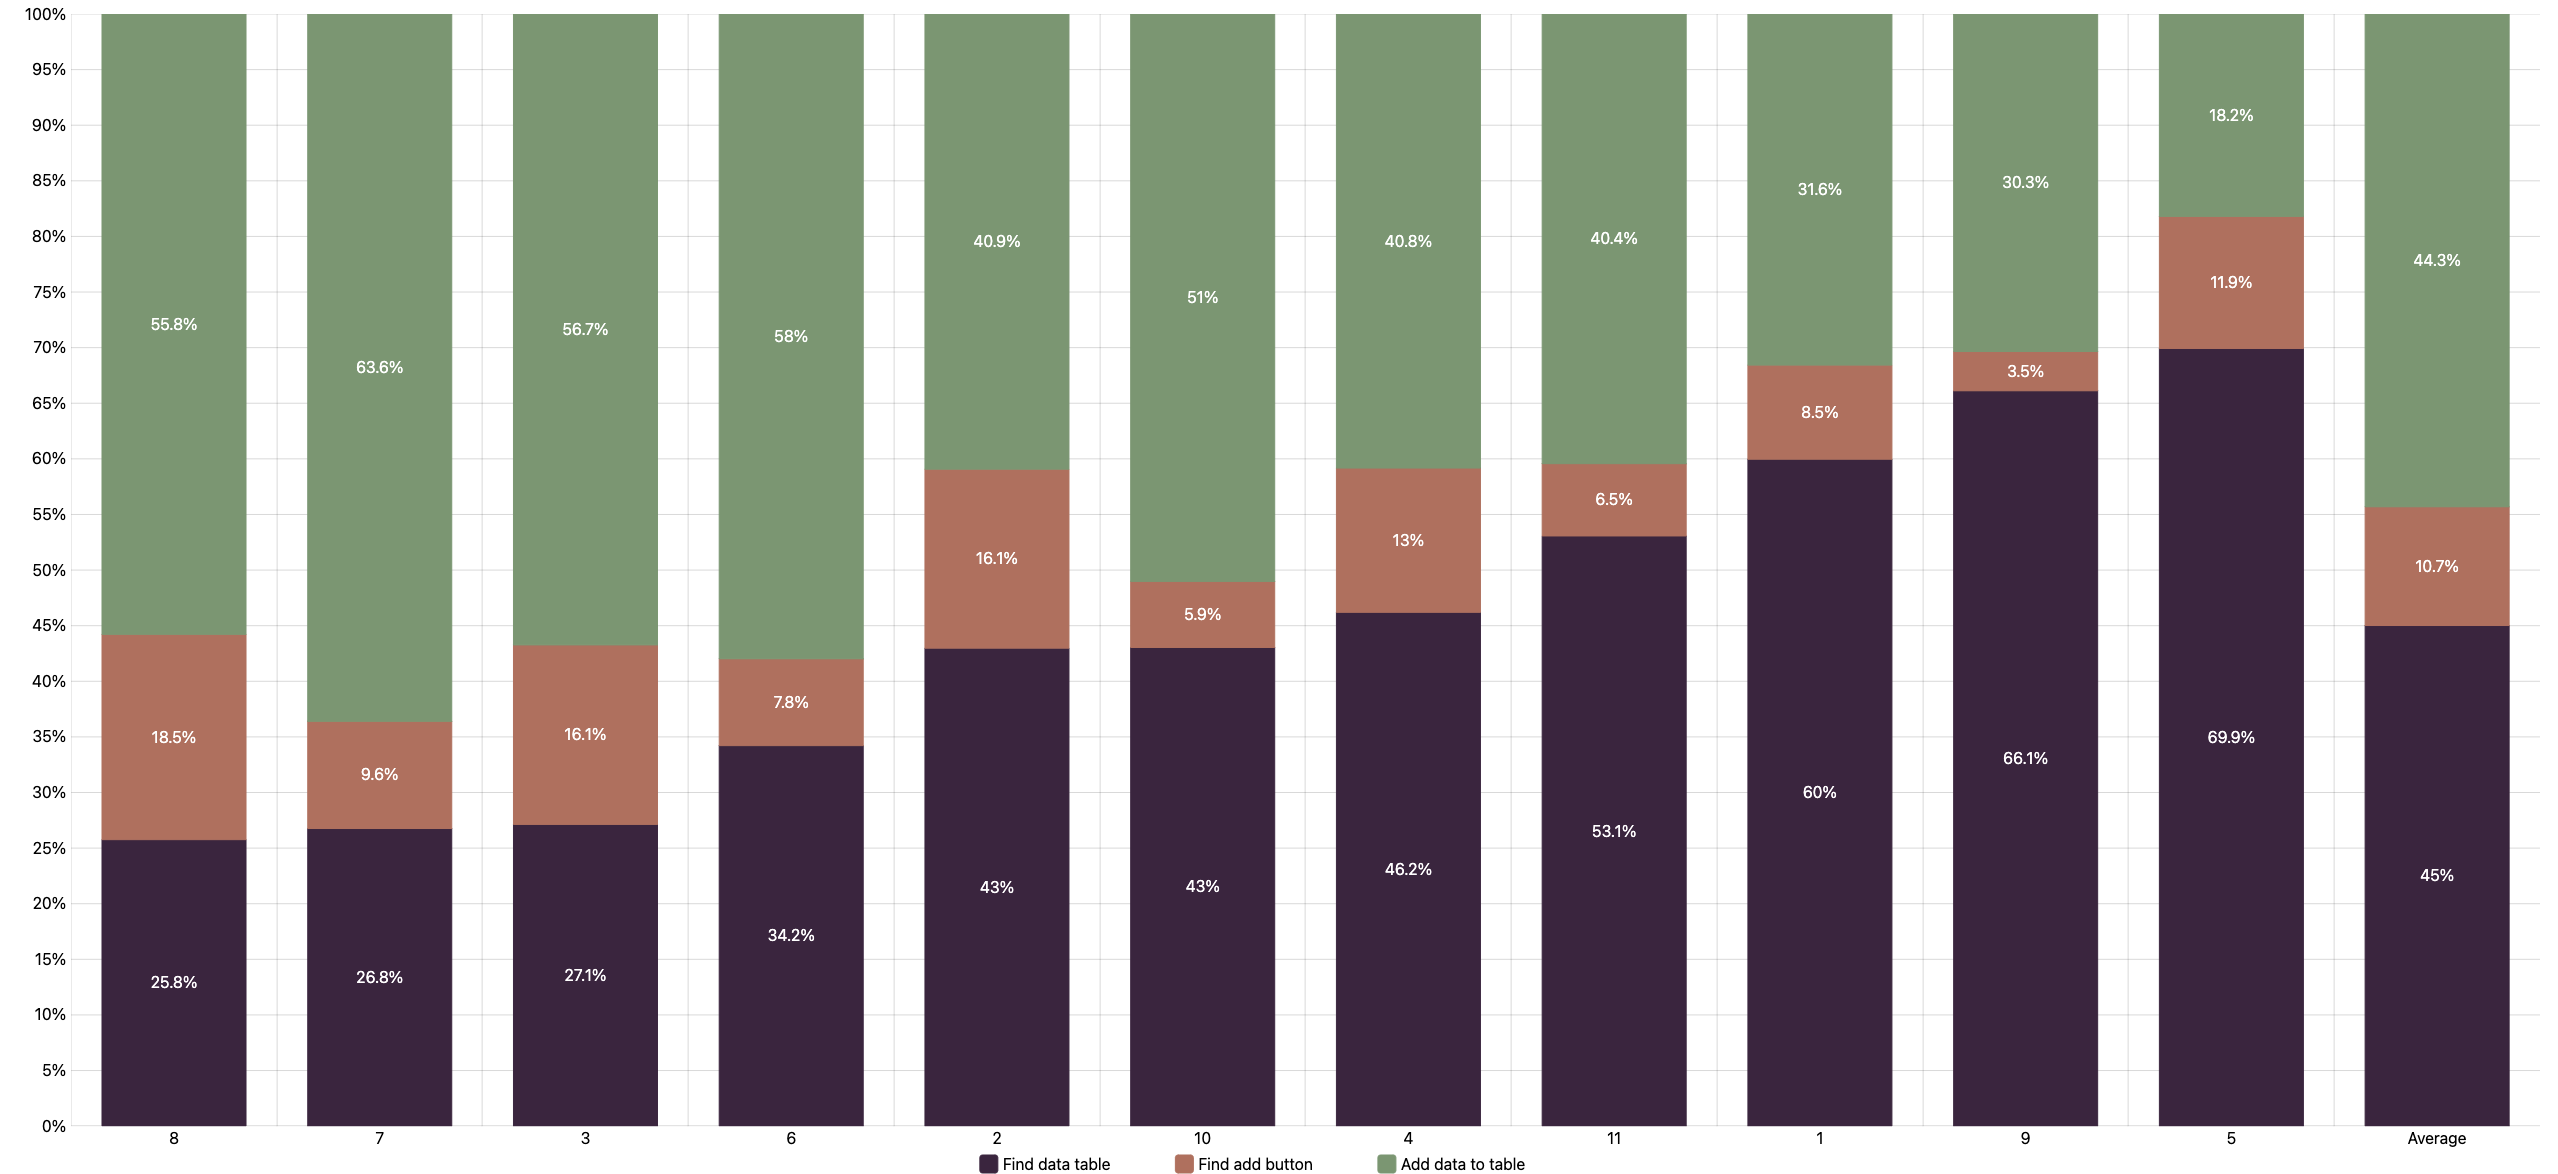
\includegraphics[width=\linewidth]{images/sds_test_data_chart.png}}
\caption{Chart of \ac{SDS} test data}
\label{test_data_sds}
\end{figure}
At first glance, Figure \ref{test_data_sds} shows the same pattern as the normal test data chart. But in closer comparison to the normal data chart (Figure \ref{test_data_normal}), the distribution of the datasets is smoother. This pattern indicates a more even distribution of the time spent on the different time windows. \\
The average column at the end of the chart shows roughly the same distribution of values as the normal data. This similarity means that finding the table of data takes, on average, the same amount of time as entering data into the form. So on average, there is no difference in the test application without \ac{SDS}. \\
As previously seen on the test sets, no runs indicate a breakout. The only interesting thing is that the search time for the "Add +" button in three test runs accounted for over 15\% of the total time. A look at test runs 8, 3, and 2 in Figure \ref{test_data_sds} shows that these tests are short overall. Therefore, a 4-second mouse movement on the button ends in a distribution of 15\% if the entire run takes only 30 seconds. However, this is not unusual user behavior in the test application.\\
Summarizing the analysis of the data chart from the test runs of SDS data, the chart shows a smoother curve which could indicate a broader group of test users. Because every user has a different interaction approach when using a tool. The chart shows the same usage patterns as in the normal test data.  \\

In order to obtain comparable test data within the test sets, it was necessary to draw a boxplot diagram. The boxplot diagram collects the total duration of each test run in one diagram. This diagram helps compare the two test sets based on the median, maximum, minimum, lower quartile, and upper quartile. \\

\begin{figure}[htbp]
    \centerline{
    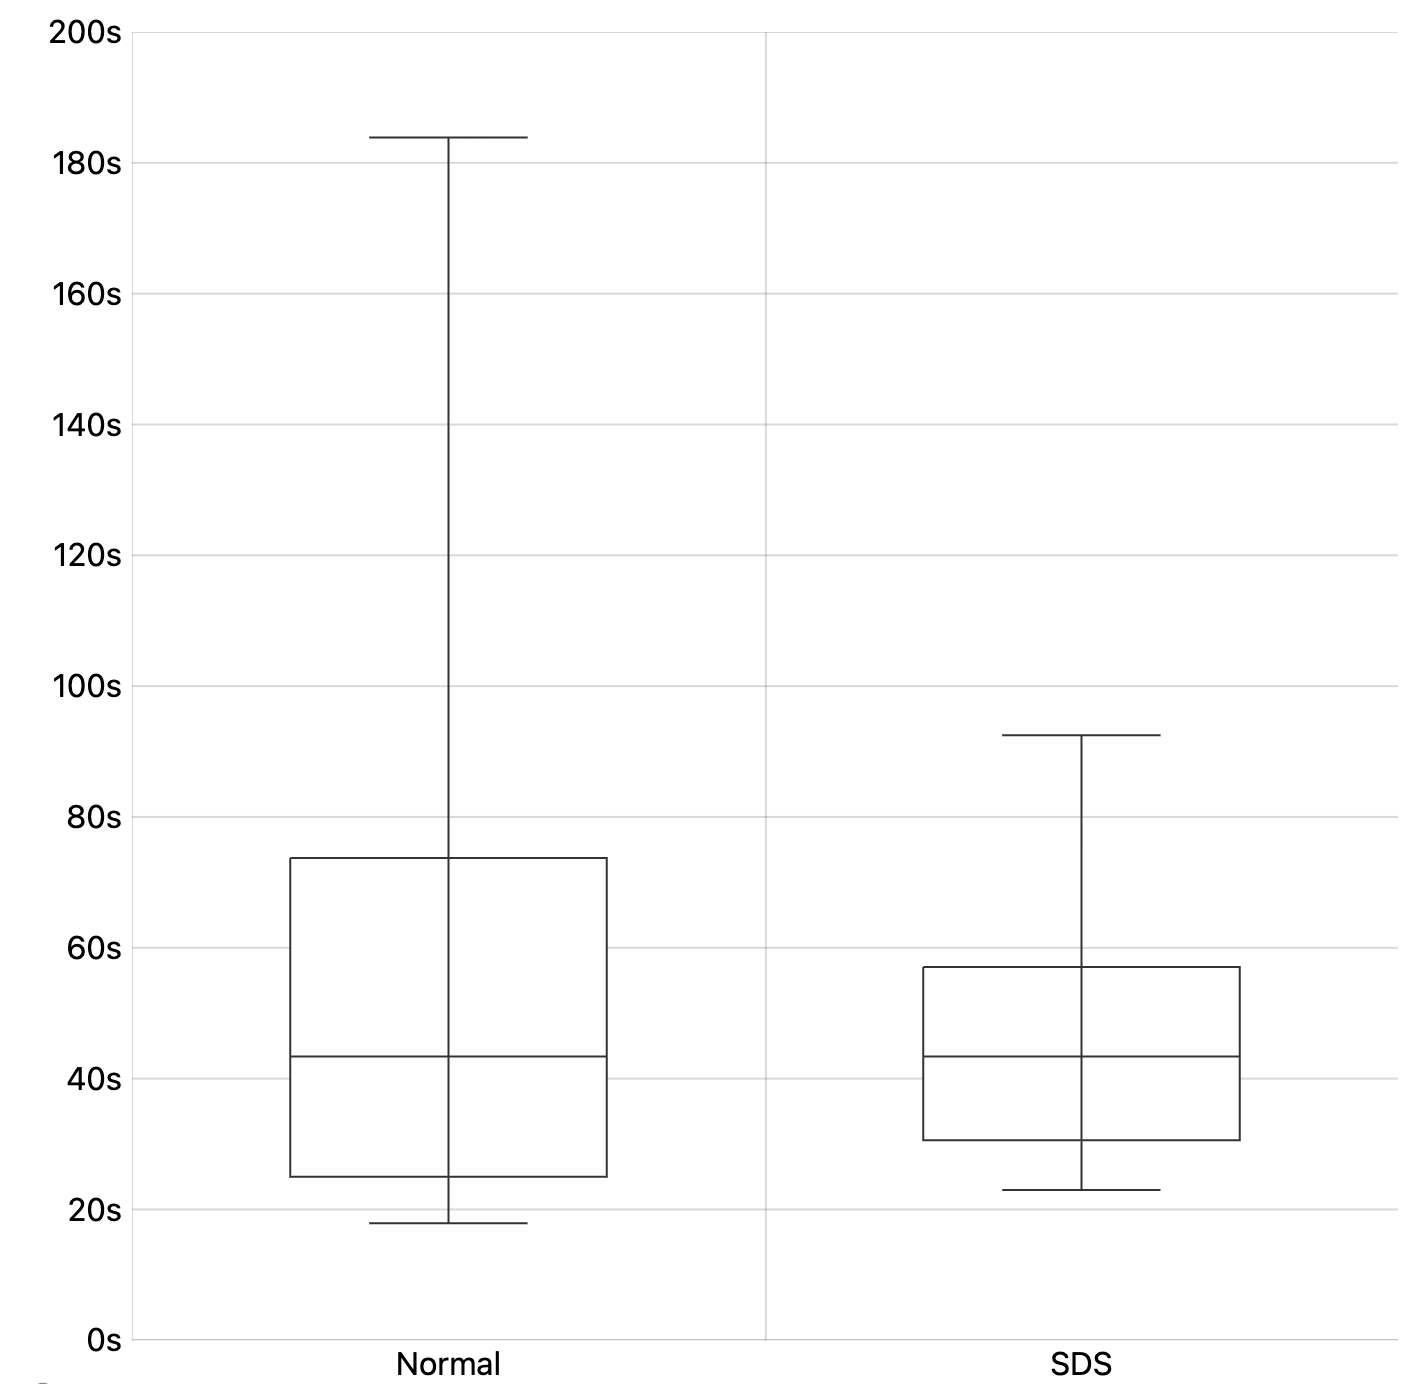
\includegraphics[height=10cm]{images/box_plot_total_duration.png}}
\caption{Boxplot diagram for comparison of both test sets based on the total duration}
\label{box_plot_comparison}
\end{figure}
Figure \ref{box_plot_comparison} shows both test sets in a boxplot diagram. The y-axis describes the total time required for the test runs in seconds. On the other Axes, the x-axis shows both test runs, the normal test run without \ac{SDS} and the test run with \ac{SDS}. \\
First, consider the two boxes in this diagram. The box for the normal test runs is larger overall than for the \ac{SDS} tests. This difference means that the runs with \ac{SDS} are closer than those without \ac{SDS}. As for the numbers, the normal test data is in the lower range of the box. The lower quartile is 24 seconds for the normal data. \\
In comparison, the \ac{SDS} box starts at 30 seconds. The end of the box for the normal test run is at 73 seconds. The \ac{SDS} box ends at 57 seconds, as explained above. It follows that 50\% of the test runs from the normal data set are between 24 and 73 seconds and correspondingly between 30 and 57 seconds for \ac{SDS}.  \\
The median shows the mean value of the test runs. The diagram represents the median with the horizontal lines inside the boxes. The values for both test runs are precisely 43 seconds. There is only a difference of 300ms. Such a tiny difference shows that the test sets do not differ in this case. \\
The last thing the chart shows are the breakdowns of each data set, represented by the vertical lines that branch off the boxes. At first glance, there is a big difference between the two data sets with the long line on one box. In the case of the normal data set, the breakouts go beyond 180 seconds. This outburst is twice as large as the highest outburst of \ac{SDS} (90 seconds). In turn, the lower bursts are not that different from the 50\% majority represented by the boxes. In both sets of tests, they look pretty similar in size. The only difference visible here is the actual value. For the normal test set, the lowest value of the test set is 17 seconds. For \ac{SDS}, this value is slightly higher at 22 seconds. Nevertheless, a difference of 5 seconds. \\
To sum it up, the chart shows a much greater variety in the test series than in the normal run. However, it also shows that the application without SDS allows users to complete their tasks faster in extreme cases but sometimes much slower. 
\subsection{Test evaluation}
The design of the tests proves the hypothesis of whether the SDS helps users complete a simple task faster than an application without \ac{SDS} implementation. After both test results presentations, it is possible to interpret the results. On the one hand, the subjective observation of each test run and, on the other hand, objective data from performance time stamps during the execution of each test run.  \\
From an observational perspective, it looks like the systems behave pretty similarly. As the results show, there are no particular patterns in either application. The observation indicates that it makes no difference with which application the user performs the task.  \\
The performance data from the test runs show a relatively similar result. In the normal test runs, there seems to be a clear division of usage patterns. For example, a user spends a relatively large amount of time finding the data table or a relatively large amount of time adding data. Compared to the \ac{SDS} test runs, the time patterns are more balanced, with a smooth transition between a long time for finding the data table and a long time for data entry. This pattern difference indicates more extremes in the runs for the normal version.  \\
In addition to this information, the boxplot diagram provides further insights. Again, the noticeable pattern in the normal test runs is visible. TThe normal data has a broader range in the boxplot than the \ac{SDS} test runs. The normal application seems to have a more random interaction pattern than the \ac{SDS} application. However, this is not all bad. The normal data run also better in terms of minimum time. The \ac{SDS} seems to help the application create a more consistent user usage pattern.  \\
In conclusion, using the \ac{SDS} helps to perform tasks more consistently and thus faster. Furthermore, the graph results show that the \ac{SDS} is generally faster. As a final step, the chi-square test evaluates whether the data points presented are statistically significant. \\

The chi-square test, according to \citeauthor{pearson_x_1900}, helps to identify whether an application is faster with \ac{SDS} than without \ac{SDS}. As the first step, a null hypothesis must be defined. In this case, the null hypothesis is whether the application with SDS implemented is faster than the normal application. The result should be significant, with a probability of 95\%. \cite{pearson_x_1900} \\ 
Since it is impossible to compare the data of each set of tests because different users performed them, a different measurement is required. Therefore, the test looks at each run and whether the required time is less than 60 seconds. Summing up the results, the table looks like this:
\begin{table}[ht]
    \centering
    \begin{tabular}{|p{0.2\linewidth} || p{0.1\linewidth}|p{0.1\linewidth}|p{0.1\linewidth}|}
        \hline
        \textbf{Total time under 60 seconds?} &\textbf{Normal}&\textbf{\ac{SDS}}&\textbf{Total} \\ \hline\hline
        \textbf{yes} & 7 & 8 & 15 \\ \hline
        \textbf{no} & 4 & 3 & 7 \\ \hline
        \textbf{Total} & 11 & 11 & 22 \\ \hline
    \end{tabular}
    \caption{\label{tab:chi-square} Aggregated test results}
\end{table}
The next step is to calculate the expected values for each variant. First, the test multiplies each test set by the sum of the results for the met criteria of both runs. Then the sum of all test runs divides the product from before. After processing all values in the table with this method, the table looks like this: 
\begin{table}[ht]
    \centering
    \begin{tabular}{|p{0.2\linewidth} || p{0.1\linewidth}|p{0.1\linewidth}|p{0.1\linewidth}|}
        \hline
        \textbf{Total time under 60 seconds?} &\textbf{Normal}&\textbf{\ac{SDS}}&\textbf{Total} \\ \hline\hline
        \textbf{yes} & 7.5 & 7.5 & 15 \\ \hline
        \textbf{no} & 3.5 & 3.5 & 7 \\ \hline
        \textbf{Total} & 11 & 11 & 22 \\ \hline
    \end{tabular}
    \caption{\label{tab:chi-square-expected} Expected test results}
\end{table}
With the expected and actual values, it is now possible to calculate the chi-square value for each entry in the table. The following formula calculates the chi-square value for each entry:
\[\chi^2=\frac{(A_{jk} - E_{jk})^2}{E_{jk}}\]

$A_{jk}$ is an entry of the actual values table, and $E_{jk}$ is a value of the expected value table. The result is a new table with all $\chi^2$ values. The table looks like this:

\begin{table}[ht]
    \centering
    \begin{tabular}{|p{0.2\linewidth} || p{0.1\linewidth}|p{0.1\linewidth}|p{0.1\linewidth}|}
        \hline
        \textbf{Total time under 60 seconds?} &\textbf{Normal}&\textbf{\ac{SDS}}&\textbf{Total} \\ \hline\hline
        \textbf{yes} & 0.03 & 0.03 & 0.06 \\ \hline
        \textbf{no} & 0.07 & 0.07 & 0.14 \\ \hline
        \textbf{Total} & 0.1 & 0.1 & 0.2 \\ \hline
    \end{tabular}
    \caption{\label{tab:chi-square-results} Chi-squared results}
\end{table}
The total $\chi^2$ value of the test data is \texttt{0.2}. The chi-square distribution table determines the degree of freedom of the table and the specified probability of the value for the statistical relevance. For this test, the value to achieve is \texttt{3.84}. Since the total value is less than the determined value, no statistically significant relationship exists between using the SDS and the total time required to complete the task. \\

Thus, the test results provide a clear statement. While the test results indicate that a design system contributes to consistency in the use of an application, the evaluation of this data concludes that the results are not statistically significant and that the SDS does not affect the performance of completing tasks in an application.
% \subsection{Discussion}
